There's a plethora of applications taking advantage of wearable tech, not all of them using the available bio sensors, ranging from basic real-time heart rate monitoring to progress tracking, to calorie measuring, and to social network sized fitness communities.

In this chapter I will research a few such applications, compare and rate them based on following criteria. \todo{add weight to individual points}
\begin{itemize}
    \item Use of IoT possibilities -- use of available sensors, data collection from the community,
    \item User fitness assessment -- how the user's fitness is assessed (attempt self-assessment, fill out a questionnaire, or take a physical test),
    \item Track difficulty assessment -- how the track's difficulty is assessed (user-reported, or calculated)
    \item Community -- built-in sharing options, possibility for interaction between users,
    \item Extra features -- interesting perks outside of the scope of my app,
    \item User-friendliness -- navigation around the mobile application - finding the general settings, creating and clearing a route, general user experience,
    \item Availability -- is the application or its parts free, paid or are there microtransactions,
    \item Cross-platform -- major operating systems supporting the mobile application and sensors, if any are used,
    \item Propriety -- whether the solution is open-source, closed-source or else.
\end{itemize}


\subsection{komoot}
The cross-platform application for outdoor track suggestion can also be used as a tour planner, a map and a navigation system.

\todo[color = green]{add numeric ratings}

\subsubsection*{Use of IoT possibilities}
Given its use of GPS sensors, komoot does qualify as a basic IoT system, however, it also relies heavily on user input for track rating.
The smart watch only gets used for displaying of routes and navigation, not taking any advantage of the available sensors.
\subsubsection*{User fitness assessment}
When a user is creating a route, they can set its difficulty as one of five levels, 
describing the user's self-reported physical fitness and their current taste for a challenge (or lack thereof): Couch Potato, Average, In Good Shape, Athletic, and Pro.
This parameter is considered when the app is generating a suitable route -- presumably by trying to adjust the elevation profile of the possible routes.
The user's real fitness is not taken into account.
\subsubsection*{Track difficulty assessment} 
Thanks to the maps provided by the OpenStreetMap, users are able to pick a starting point, a destination, as well as any number of waypoints in between for their route.
Once the route is chosen, the user can go through the route's stats - the estimated time it will take to get from start to finish, its length, the elevation profile (uphill, downhill, highest and lowest points, estimated average speed) and the surfaces and their use in proportion to the route's length.
All this information is delivered in easy-to-understand charts as well as interactive mappings -- using a slider, the user can see which stat applies in which part of the route.

\begin{figure}[h]
    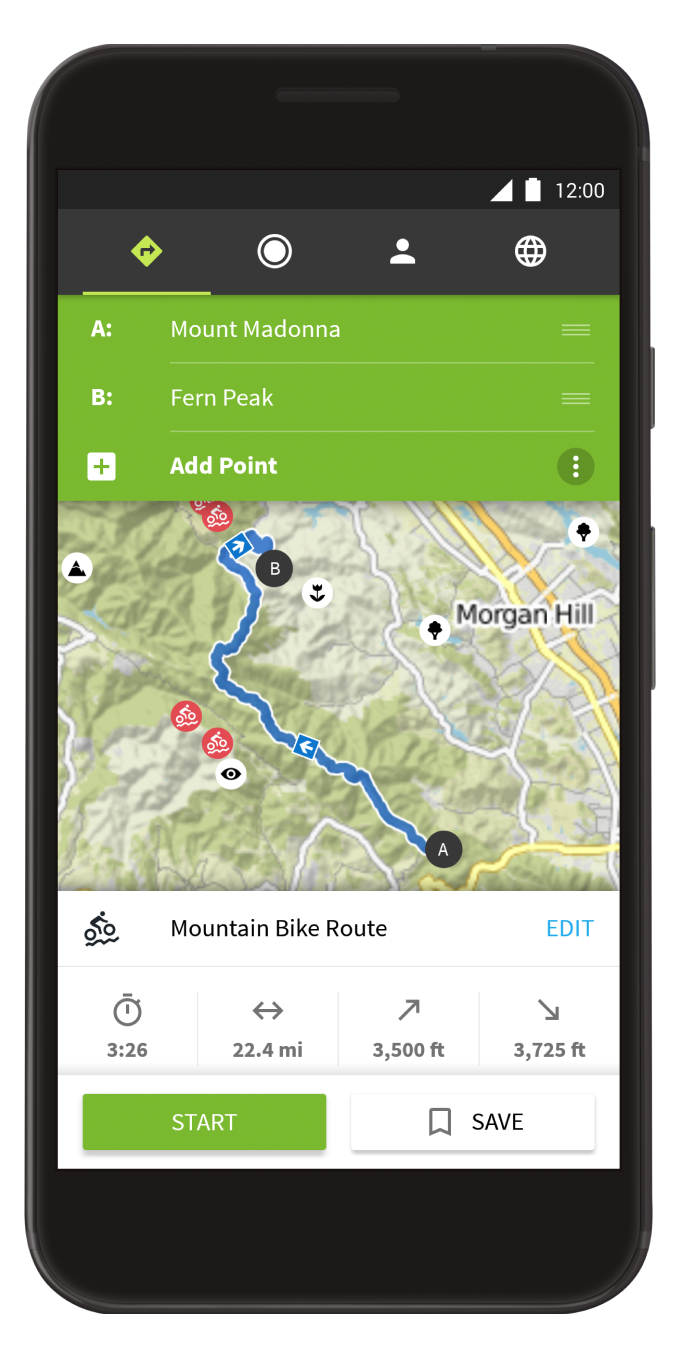
\includegraphics[width=\textwidth]{komoot-nav.png}
    \caption{Offline maps in the komoot app\cite{komoot-nav-img}}
\end{figure}

\begin{figure}[h]
    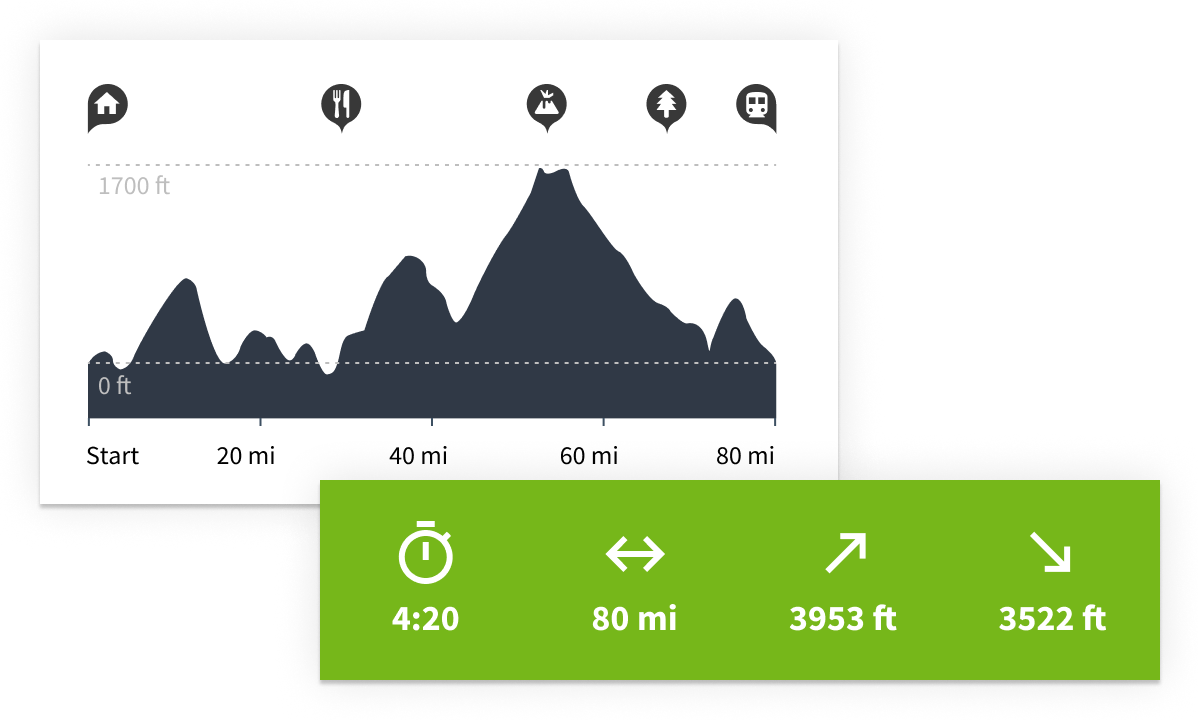
\includegraphics[width=\textwidth]{komoot-route-details.png}
    \caption{Route elevation profile\cite{komoot-route-details-img}}
\end{figure}

\begin{figure}[h]
    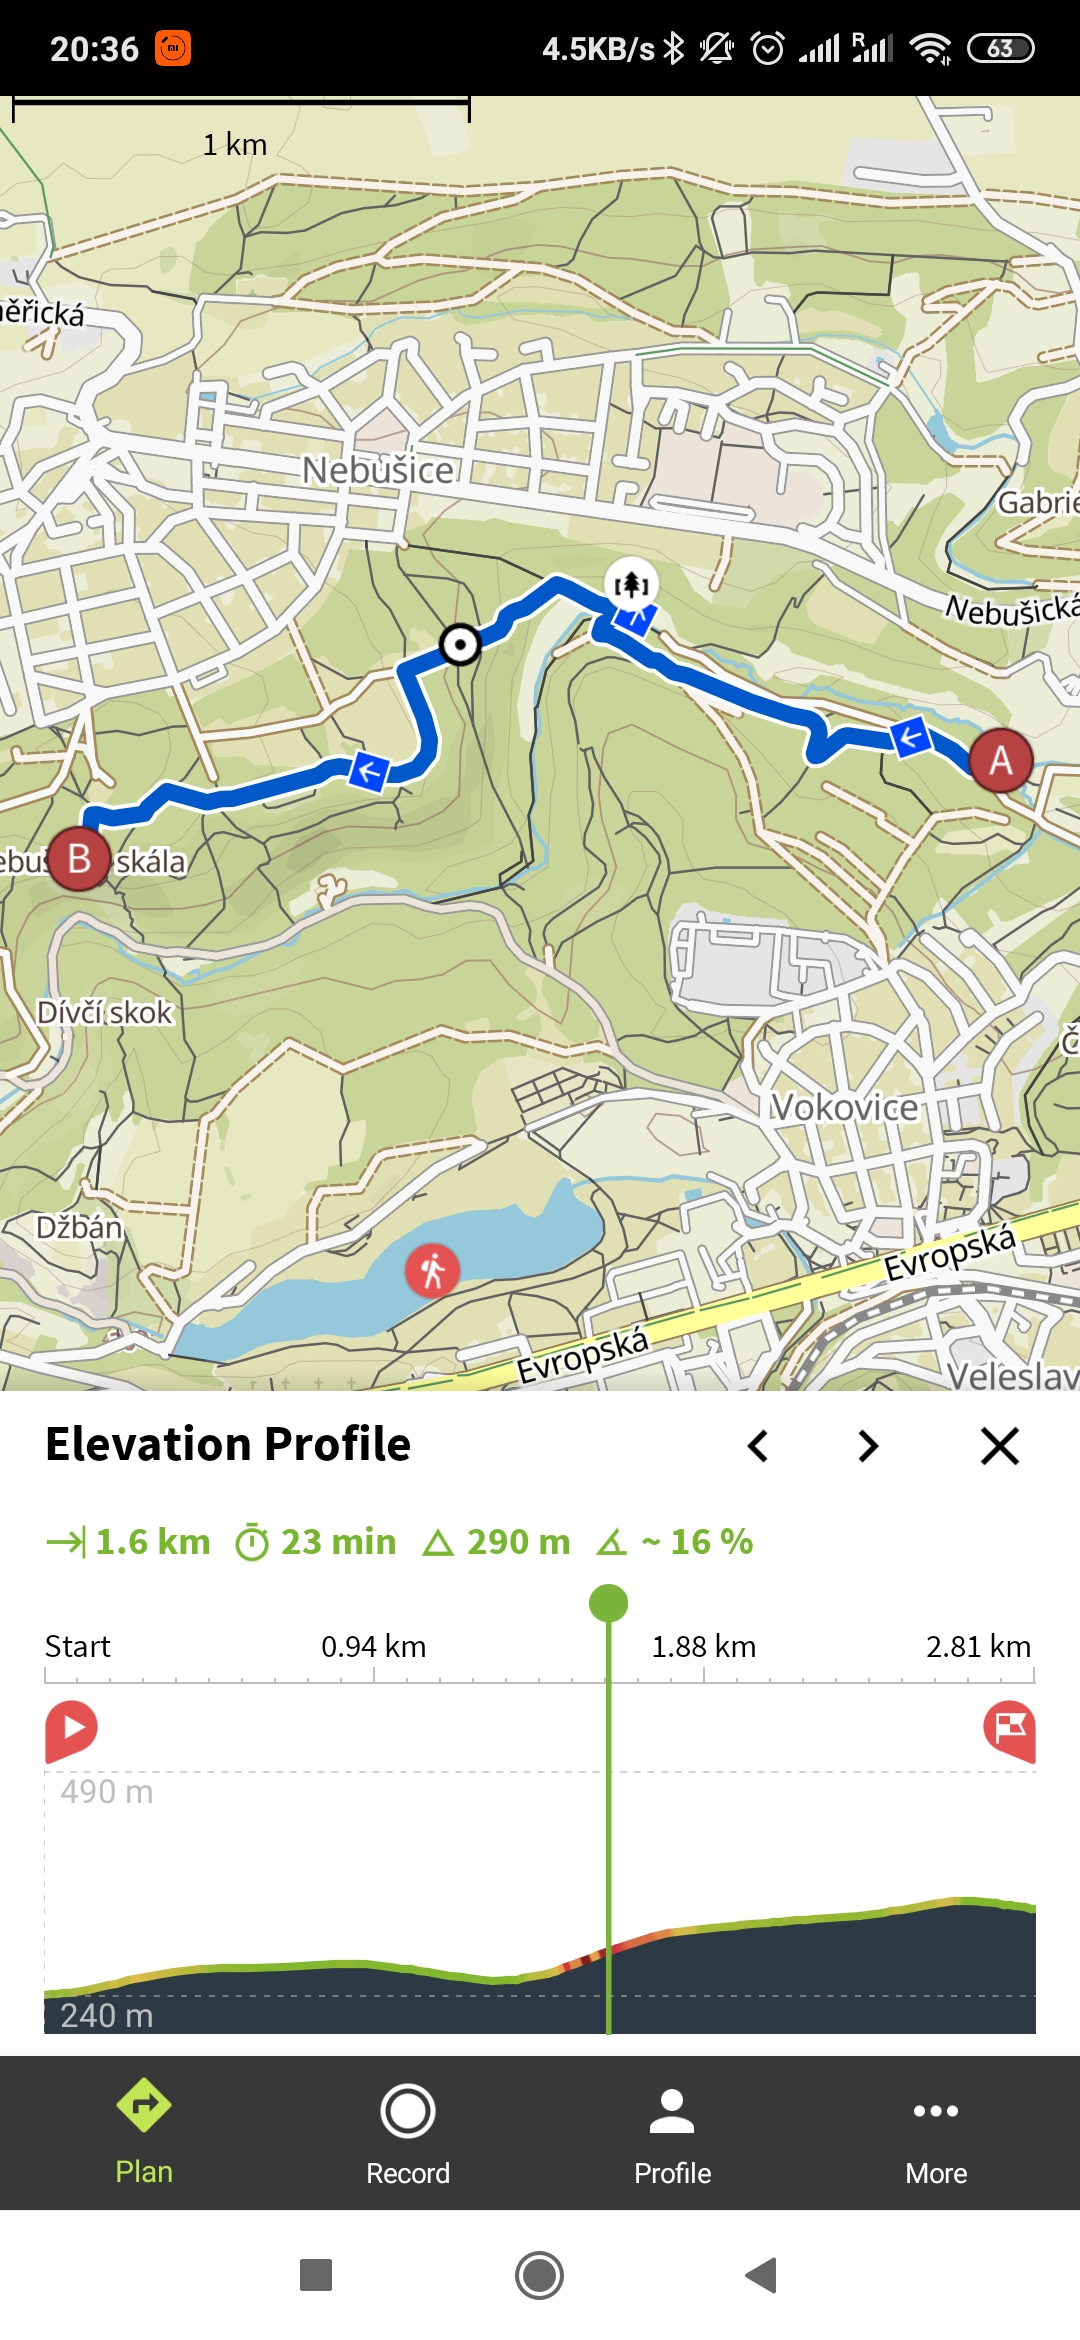
\includegraphics[width=\textwidth]{komoot-route-elevation-detail.jpg}
    \caption{Detailed view of the route's elevation\cite{komoot-route-elevation-detail-img}}
\end{figure}

\begin{figure}[h]
    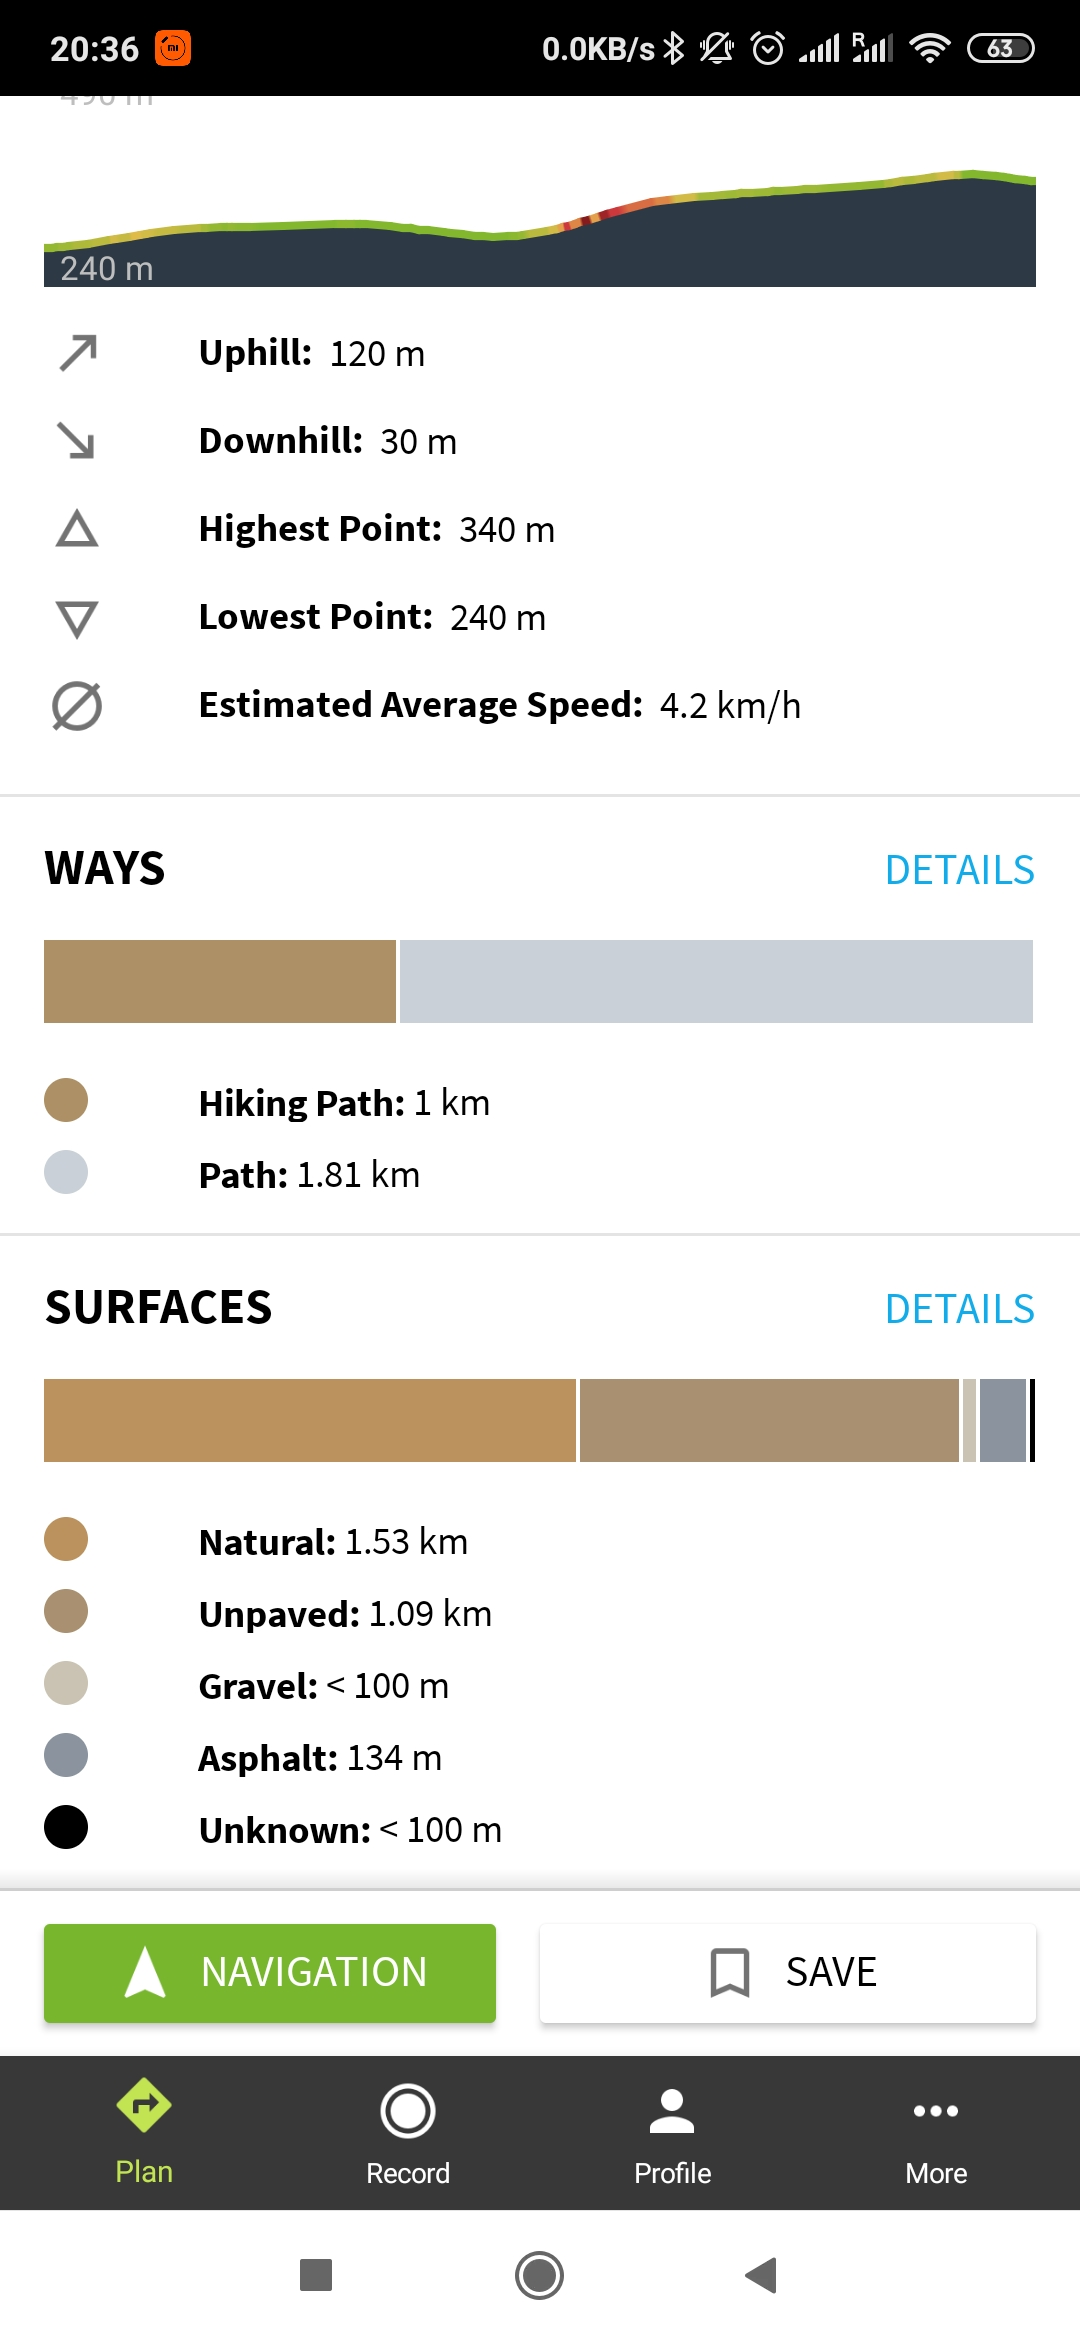
\includegraphics[width=\textwidth]{komoot-route-surface-detail.jpg}
    \caption{Overview of the route's surface. The detailed view is similar to the elevation detail.\cite{komoot-route-surface-overview-img}}
\end{figure}


\subsubsection*{Availability}
The region-based pricing model allows users who do not travel too much to use the app for free,
since the first region is provided at no cost.
In the other pricing options Single Region, Region Bundle and All Regions -- the price-performance ratio seems to grow at a reasonable scale.\todo[color = green]{anything to add?}
\subsubsection*{Community}
With features like sharing of routes users have taken, following of other users, upvoting and commenting on their posts, the mobile application integrates a full-fledged social network.
\subsubsection*{Extra features}

\subsubsection*{User-friendliness}
The navigation through the mobile app takes some time to get used to -- it took me a while to find the Settings after I didn't see them in the burger menu on the bottom navigation bar, which contained only the different pricing options.
Once I created a route, the information provided was well-delivered and easy to read, however, there was no obvious way of completely cancelling the chosen route and picking another one.
Instead, hiding in the Options of the route -- which at first I didn't even notice -- I found the "Reset route" option, which did just what I needed.
Overall, the app has some great parts and some not-so-great ones.
\subsubsection*{Cross-platform}
The system is fully integrated with the Apple Watch and Samsung gear, and -- at least limitedly -- supports a number of other brands of smart watches and other Bluetooth-enabled devices.
The mobile application runs both on iPhones and Android phones.
\subsubsection*{Propriety}
The system is not entirely open-source, as a few of their repositories are public, but the core components remain proprietary. \todo[color = green]{recheck}\todo[color = green]{cite https://github.com/komoot}

\subsubsection*{Overall evaluation}
While being rich with features, komoot doesn't base its functionality on objective data -- it's the users themselves who rate and recommend the specific routes,
an approach in its nature prone to error and with only limited ways of eliminating the human factor.

\subsection{endomondo}
https://www.endomondo.com/
\subsubsection*{Use of IoT possibilities} --
\subsubsection*{User fitness assessment} --
\subsubsection*{Availability} --
\subsubsection*{Community} -- 
\subsubsection*{Extra features} -- 
\subsubsection*{User-friendliness} -- 
\begin{figure}[h]
    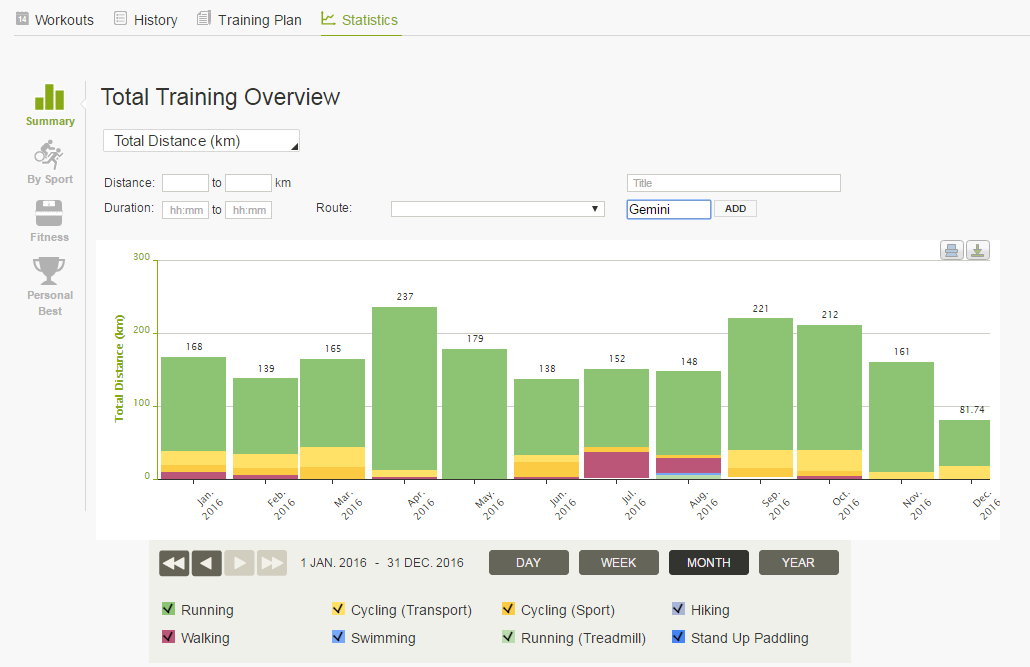
\includegraphics[width=\textwidth]{endomondo-history-example.png}
    \caption{endomondo history example\cite{endomondo-history-img}}
\end{figure}

\begin{figure}[h]
    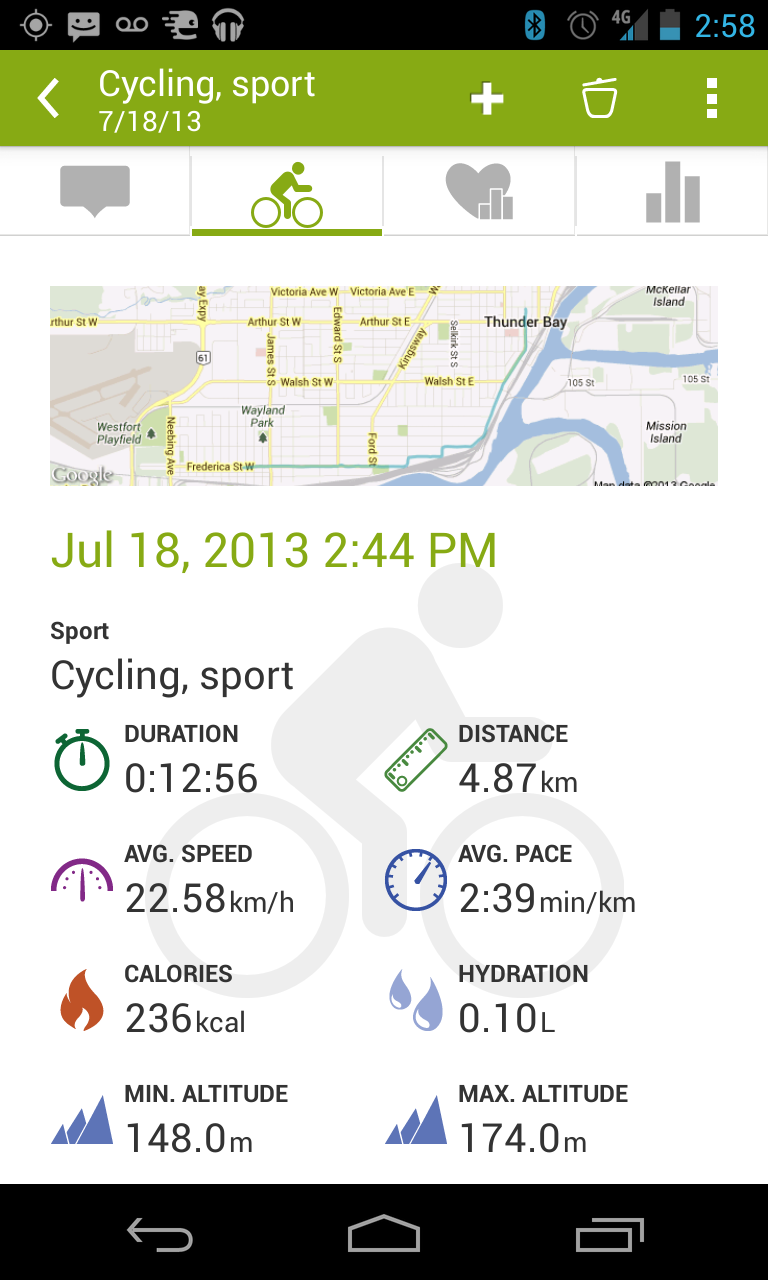
\includegraphics[width=\textwidth]{endomondo-bike-stats.png}
    \caption{Statistics of a biking trip on endomondo\cite{endomondo-bike-stats-img}}
\end{figure}

\subsubsection*{Cross-platform} -- 
\subsubsection*{Propriety} -- 
\subsubsection*{Overall evaluation}

\subsection{Strava}
https://www.strava.com/
\subsubsection*{Use of IoT possibilities} --
\subsubsection*{User fitness assessment} --
\subsubsection*{Availability} --
\subsubsection*{Community} -- 
\subsubsection*{Extra features} -- 
\subsubsection*{User-friendliness}
\begin{figure}[h]
    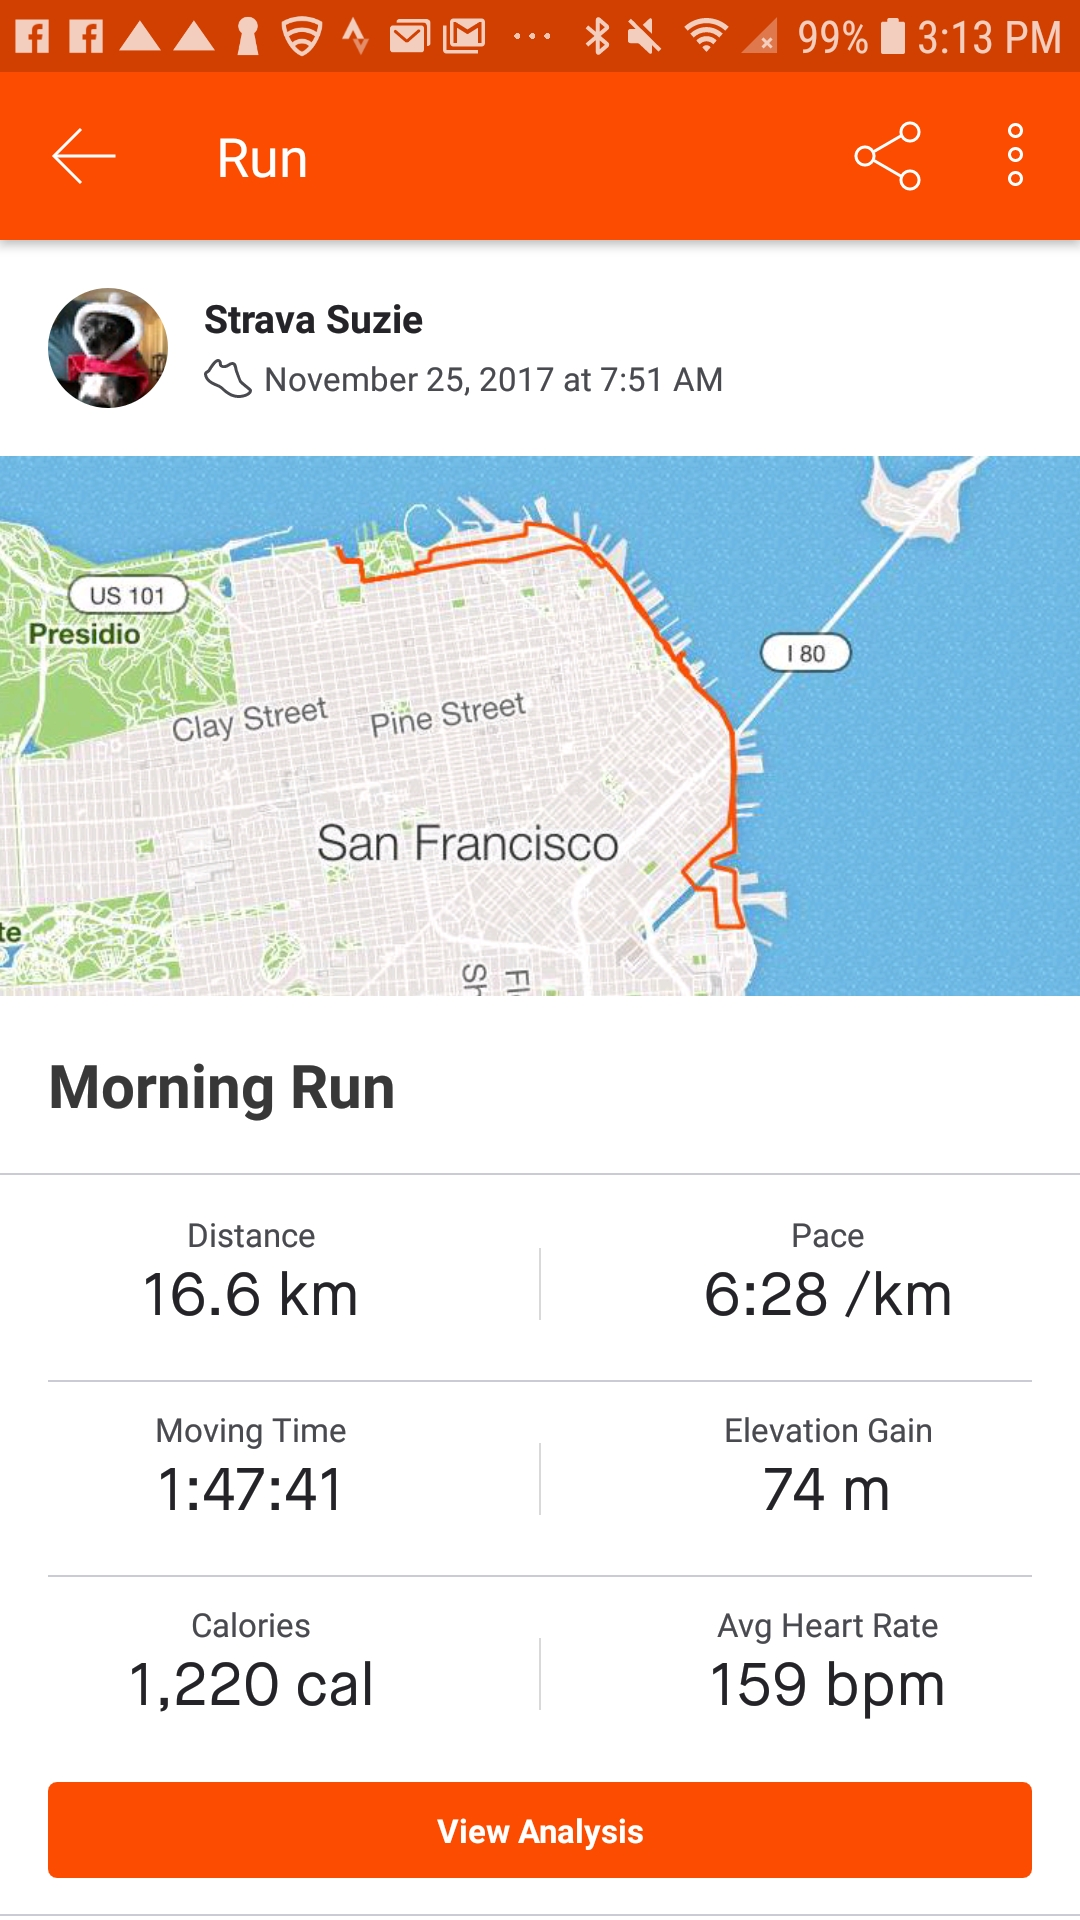
\includegraphics[width=\textwidth]{strava-morning-run-stats.jpg}
    \caption{Statistics of a run on strava\cite{strava-run-stats-img}}
\end{figure}
\subsubsection*{Cross-platform} -- 
\subsubsection*{Propriety} -- 
\subsubsection*{Overall evaluation}

\subsection{myFitnessPal}
https://www.myfitnesspal.com/
\subsubsection*{Use of IoT possibilities} --
\subsubsection*{User fitness assessment} --
\subsubsection*{Availability} --
\subsubsection*{Community} -- 
\subsubsection*{Extra features} -- 
\subsubsection*{User-friendliness} -- 

\begin{figure}[h]
    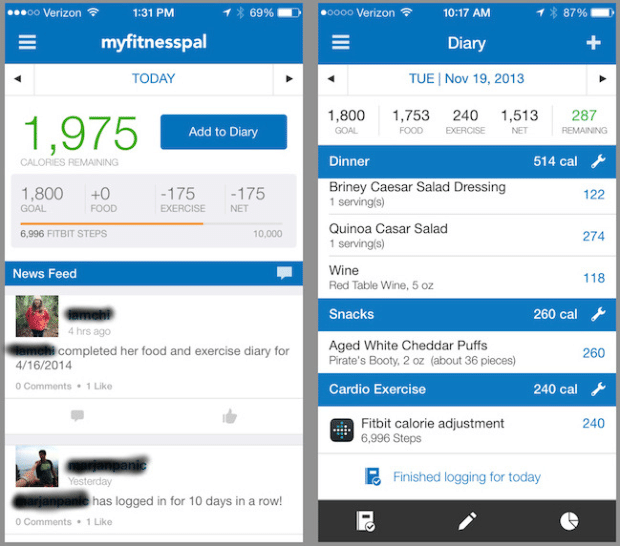
\includegraphics[width=\textwidth]{myfitnesspal-researchgate.png}
    \caption{myFitnessPal feed and diary entry\cite{MFP-diary-img}}
\end{figure}

\subsubsection*{Cross-platform} -- 
\subsubsection*{Propriety} -- 
\subsubsection*{Overall evaluation}

\subsection{Walk with Map My Walk}
https://www.mapmywalk.com/
\subsubsection*{Use of IoT possibilities} --
\subsubsection*{User fitness assessment} --
\subsubsection*{Availability} --
\subsubsection*{Community} -- 
\subsubsection*{Extra features} -- 
\subsubsection*{User-friendliness} -- 

\begin{figure}[h]
    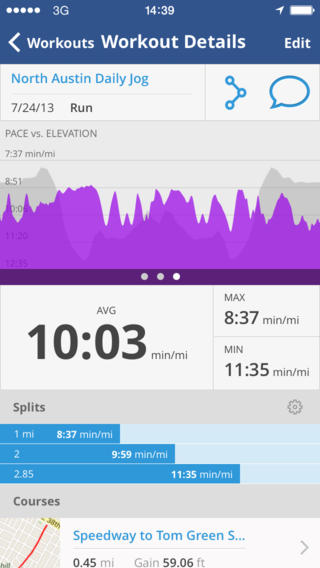
\includegraphics[width=\textwidth]{map-my-fitness-workout-details.jpg}
    \caption{Map my Fitness workout details\cite{map-my-walk-img}}
\end{figure}


\subsubsection*{Cross-platform} -- 
\subsubsection*{Propriety} -- 
\subsubsection*{Overall evaluation}

\subsection{Garmin Explore and Garmin Connect}
The vast ecosystem Garmin has created for their users is filled with an assortment of wearables, radars, smart lights, navigations, customized maps, and plenty more, providing features which are presented to the user via modular mobile apps.

Here I will analyse the Garmin Explore application, which is targeted at hikers, in tandem with Garmin Connect, which functions as a fitness tracker.

\subsubsection*{Use of IoT possibilities}
Most fitness-focused Garmin watches do have a heart rate sensor and all of them include a step counter, however, this data is never compared with that of other users, keeping focus on the user's activity history with no prediction.
\subsubsection*{User fitness assessment}
Some of the heart-rate-monitor enabled watches allow a user to set the zones in which they would like to keep their heart rate depending on the activity they choose to do. The standard zones are:
\textit{
\begin{itemize}
    \item Zone 1 (Warm Up) --
    Perceived exertion: Relaxed, easy pace, rhythmic breathing. Benefits: Beginning-level aerobic training, reduces stress.
    \item Zone 2 (Easy) --
    Perceived exertion: Comfortable pace, slightly deeper breathing, conversation possible. Benefits: Basic cardiovascular training, good recovery pace.
    \item Zone 3 (Aerobic) --
    Perceived exertion: Moderate pace, more difficult to hold conversation. Benefits: Improved aerobic capacity, optimal cardiovascular training.
    \item Zone 4 (Threshold) --
    Perceived exertion: Fast pace and a bit uncomfortable, breathing forceful. Benefits: Improved anaerobic capacity and threshold, improved speed.
    \item Zone 5 (Maximum) --
    Perceived exertion: Sprinting pace, unsustainable for long period of time, labored breathing. Benefits: Anaerobic and muscular endurance, increased power.\cite{garmin-heart-zones}
\end{itemize}
}

\begin{figure}[h]
    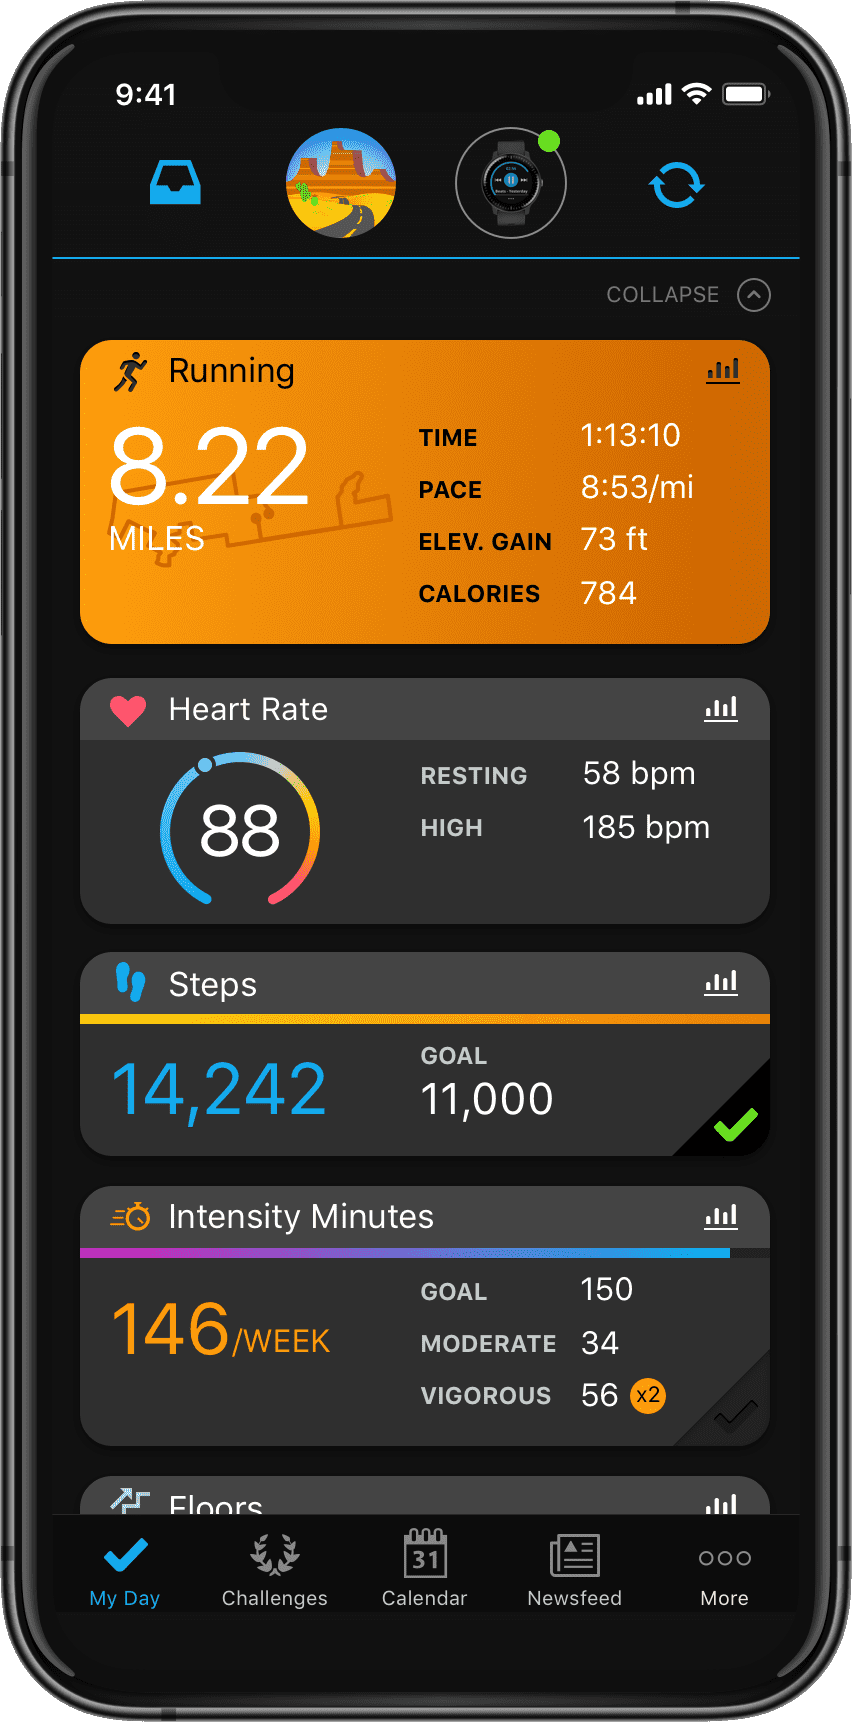
\includegraphics[width=\textwidth]{garmin-connect-myday-screen.png}
    \caption{My day - Garmin Connect's home screen displays statistics of the user's recent activity\cite{garmin-my-day-img}}
\end{figure}

\subsubsection*{Track difficulty assessment}

\subsubsection*{Availability}
In general, Garmin's pricing model relies on the user buying one of their high-end smartwatches, whereupon the rest of the components (apps, basic maps, support, etc.) are free, with some exceptions, such as advanced maps. 
The company's smartwatches are considered premium quality, with a wide price range - target groups include \textit{potential Rolex buyers}\cite{garmin-expensive} as well as ordinary users.\cite{garmin-watches-review}
\subsubsection*{Community}
The Connect application handles the data from the point of view of a fitness tracker, with social features like groups, competitions, likes, comments, and badges of accomplishment.\cite{garmin-connect}
\subsubsection*{Extra features} -- 
\subsubsection*{User-friendliness}

\subsubsection*{Cross-platform}
All of Garmin's applications can be installed both on Android and iPhone.
However, they can only be paired with watches inside Garmin's ecosystem, which is a drawback for users who already own a smartwatch.
\subsubsection*{Propriety}
Some of the Garmin applications are completely open-source, either due to the software that they are derived from, or simply to provide the general public with opportunity to customize their Garmin experience.\cite{garmin-open-source}\cite{garmin-connect-github-repos}
These apps are mostly concerned with map handling, navigation and sound codecs, but also include some bits of functionality like widgets, low power watch apps and others.

While some of this code may be used in the Explore or Connect applications, these repositories don't contain their core functionality.

\subsubsection*{Overall evaluation}
As a fitness tracker, Garmin Connect can definitely be considered acceptable...
